\subsection{Level Sets, Projections, and Apparent Orbital Geometry}
  \label{app:level_sets_orbitals}

  This appendix clarifies a general geometric property of continuous scalar fields that is
  relevant to the interpretation of atomic orbitals as threshold-visible structures.
  The results presented here are purely mathematical and do not rely on any specific physical
  interpretation.

  Level sets of $\chi$ are introduced solely as mathematical visualization tools.
  They do not correspond to fundamental spatial structures, but provide a convenient
  means of characterizing regions of comparable relaxation state in effective geometric
  descriptions.

  \subsubsection{Level Sets of Continuous Scalar Fields}

    Let $\phi : \mathbb{R}^3 \rightarrow \mathbb{R}$ be a continuous scalar field.
    For a given constant $c \in \mathbb{R}$, the corresponding level set (or isosurface) is defined as
    \begin{equation}
      \mathcal{L}_c = \{ \mathbf{x} \in \mathbb{R}^3 \mid \phi(\mathbf{x}) = c \}.
    \end{equation}

    If $\phi$ is smooth, $\mathcal{L}_c$ is generically a two-dimensional surface, possibly composed
    of several disconnected components.
    Such level sets are commonly used to visualize scalar fields by displaying only regions where
    $\phi$ exceeds a fixed threshold.

  \subsubsection{Projection-Induced Apparent Discontinuities}

    Consider the projection of $\mathcal{L}_c$ onto a single spatial coordinate, say $z$.
    Define the projected set
    \begin{equation}
      P_c = \{ z \in \mathbb{R} \mid \exists (x,y) \in \mathbb{R}^2 \text{ such that } \phi(x,y,z) \ge c \}.
    \end{equation}

    Even when $\phi$ is continuous, $P_c$ generally consists of a union of disjoint intervals.
    These intervals correspond to regions where the level set intersects planes of constant $z$.

    This projection-induced fragmentation is illustrated schematically in Fig.~\ref{fig:levelset_projection}.

  \begin{figure}[t]
      \centering
      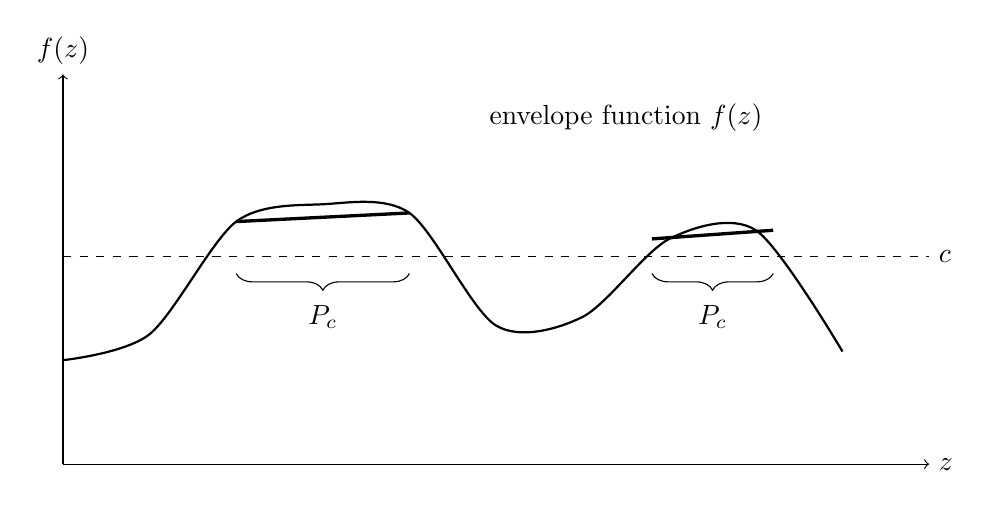
\begin{tikzpicture}[scale=1.1]

% Axes
        \draw[->] (0,0) -- (10,0) node[right] {$z$};
        \draw[->] (0,0) -- (0,4.5) node[above] {$f(z)$};

% Envelope function f(z)
        \draw[thick, smooth]
        plot coordinates {
          (0,1.2)
          (1,1.5)
          (2,2.8)
          (3,3.0)
          (4,2.9)
          (5,1.6)
          (6,1.7)
          (7,2.6)
          (8,2.7)
          (9,1.3)
        };

% Threshold
        \draw[dashed] (0,2.4) -- (10,2.4)
        node[right] {$c$};

% Highlight projected intervals
        \draw[very thick] (2.0,2.8) -- (4.0,2.9);
        \draw[very thick] (6.8,2.6) -- (8.2,2.7);

% Braces for Pc
        \draw[decorate,decoration={brace,mirror,amplitude=6pt}]
        (2.0,2.2) -- (4.0,2.2)
        node[midway,below=8pt] {$P_c$};

        \draw[decorate,decoration={brace,mirror,amplitude=6pt}]
        (6.8,2.2) -- (8.2,2.2)
        node[midway,below=8pt] {$P_c$};

% Labels
        \node at (6.5,4.0) {envelope function $f(z)$};

      \end{tikzpicture}
      \caption{Projection-induced apparent discontinuities.
      The envelope function $f(z)=\max_{x,y}\phi(x,y,z)$ is continuous, but the projected set
        $P_c=\{z\mid f(z)\ge c\}$ consists of disjoint intervals.
        The apparent fragmentation results from thresholding and does not reflect any
        discontinuity of the underlying scalar field $\phi$.}
      \label{fig:levelset_projection}
    \end{figure}

    Importantly, the apparent disjointness of $P_c$ does not imply any discontinuity of the underlying
    field $\phi$.
    Rather, it arises from the fact that only regions exceeding the chosen threshold $c$ are retained.
    The fragmentation is therefore a projection effect induced by thresholding.

  \subsubsection{Envelope Function and Threshold Visibility}

    Define the envelope function
    \begin{equation}
      f(z) = \max_{x,y} \phi(x,y,z).
    \end{equation}

    The set $P_c$ can then be written equivalently as
    \begin{equation}
      P_c = \{ z \in \mathbb{R} \mid f(z) \ge c \}.
    \end{equation}

    The function $f(z)$ is uniquely determined by $\phi$ and provides a global one-dimensional
    summary of the field's maximal amplitude along each slice of constant $z$.
    While the full three-dimensional structure of $\phi$ cannot be reconstructed from $P_c$ alone,
    the envelope function $f(z)$ encodes the emergence and disappearance of visible components as the
    threshold $c$ is varied.

    In this sense, threshold-based visualizations reveal sections of a continuous structure rather
    than discrete or independent objects.

  \subsubsection{Non-Uniqueness of Inverse Reconstruction}

    Given a projected set $P_c$ or a collection of disjoint level-set components, the inverse problem
    of reconstructing $\phi$ is not uniquely solvable.
    Multiple continuous scalar fields may share identical level sets at a given threshold.

    Additional assumptions---such as symmetry, minimal curvature, smoothness, or governing differential
    equations---are required to select a preferred reconstruction.
    The present result therefore establishes a structural constraint rather than a unique inversion.

  \subsubsection{Summary}

    Level-set visualizations of continuous scalar fields generically produce apparently disjoint
    structures when projected or thresholded.
    These structures should be understood as emergent sections of an underlying continuous field.
    The mathematical origin of this effect is independent of any specific physical interpretation,
    but it provides a natural geometric framework for understanding disjoint orbital-like patterns
    as manifestations of threshold visibility.

    While this appendix is presented independently of any physical model, the
    results apply directly to situations in which observable structures are
    defined by detection thresholds or projection procedures, as in atomic,
    optical, or imaging contexts.

    These effects are purely geometric and arise generically whenever continuous scalar
    fields are visualized through threshold-based projections (see Fig.~\ref{fig:levelset_projection}).
